
% \documentclass[11pt]{article}

% % ---------- PACKAGES ----------
% \usepackage[a4paper,margin=1in]{geometry}
% \usepackage{graphicx}
% \usepackage{amsmath,amssymb}
% \usepackage{microtype}
% \usepackage{booktabs}
% \usepackage{hyperref}
% \usepackage{cleveref}
% \usepackage{xcolor}
% \usepackage{siunitx}
% \usepackage{titlesec}

% \titleformat{\section}{\large\bfseries}{\thesection}{0.5em}{}
% \titleformat{\subsection}{\normalsize\bfseries}{\thesubsection}{0.5em}{}
% \titleformat{\subsubsection}{\normalsize\itshape}{\thesubsubsection}{0.5em}{}

% \title{\textbf{Procedural and Learning-Based Generation of Coral Reef Islands}}
% \author{[Author Names and Affiliations]}
% \date{}

% \begin{document}
% \maketitle

% \begin{abstract}
% We present a hybrid procedural and deep-learning method for generating coral reef island terrains that are geologically plausible, controllable, and fast to synthesize. Our approach procedurally constructs labeled height maps from user sketches---top-view outlines, a 1D elevation profile, and stroke-based wind/wave fields---and uses these synthetic pairs to train a conditional GAN (pix2pix). The trained model maps semantic label maps (with subsidence encoded) to height fields in real time. This framework merges procedural structure with learned realism, enabling interactive creation of diverse reef islands at $256\times256$ resolution without real-world DEMs.
% \end{abstract}

\resetgraphicspath
\appendtographicspath{{./Chapter 1/figures/} }
\appendtographicspath{{./Chapter 1/figures/Procedural/} }
\appendtographicspath{{./Chapter 1/islands/} }
\appendtographicspath{{./Chapter 1/Results/} }
\appendtographicspath{{./Chapter 1/Results/Procedural/} }
\appendtographicspath{{./Chapter 1/Results/Reproduction/} }
\appendtographicspath{{./Chapter 1/Results/results_cGAN_PG25/} {./Chapter 1/Results/results_cGAN_PG25/Renders} }
\appendtographicspath{{./Chapter 1/Results/volcanic/} }
\appendtographicspath{{./Chapter 1/figures/Smoothmax/} }
\appendtographicspath{{./Chapter 1/figures/vector_field/} }
\appendtographicspath{{./Chapter 1/figures/SOTA/coral theories/} }
\appendtographicspath{{./Chapter 1/figures/SOTA/sketching/} }

\section{Introduction}

Coral reef islands emerge from long-term interplay between volcanic uplift/subsidence, coral growth, erosion, and hydrodynamics, which complicates procedural modeling and limits available training data. Noise-based terrains lack biological/geological grounding; physically-based simulators are costly and tailored to continental processes; deep models require data that are scarce for reefs.
%
We address this by combining \emph{sketch-based procedural generation} with a \emph{conditional generative model}: a user draws concentric region outlines (island, beach, lagoon, reef, abyss) and a 1D elevation profile; stroke-based wind fields deform the island. We emulate subsidence and coral ``keep-up'' growth procedurally, then train a pix2pix cGAN on the resulting (label map, height field) pairs. At inference, users provide a semantic label image; the model yields a plausible height map.

\paragraph{Geological framing (one paragraph).}
We adopt Darwin's subsidence theory~\cite{Darwin1842} as a simple, effective basis: fringing reefs transform to barrier reefs and atolls as a volcanic island slowly sinks, with corals maintaining elevation near the photic zone (see also~\cite{Terry2013}). Competing hypotheses (e.g., Murray's stand-still~\cite{Murray1880}, Daly's glacial control~\cite{Daly1915}, Droxler's karstification~\cite{Droxler2021}) inform our assumptions but are beyond scope for our generator.

\paragraph{Contributions.} (i) a sketch-based procedural algorithm combining dual-view sketches with stroke-driven deformation and resistance; (ii) a procedural model of subsidence and analytic coral growth blended via a smooth maximum; (iii) a synthetic dataset pipeline that encodes labels and subsidence in HSV for cGAN training; (iv) a demonstration that standard pix2pix trained on procedural data produces plausible coral islands from rough user sketches in real time.

\begin{figure}[t]
  \centering
  \includegraphics[width=\linewidth]{pipeline_full.pdf}
  \caption{Pipeline overview: sketch input $\rightarrow$ procedural synthesis (height + labels) $\rightarrow$ dataset augmentation $\rightarrow$ cGAN training $\rightarrow$ real-time generation from semantic label maps.}
  \label{fig:pipeline}
\end{figure}

\section{Related Work}

\paragraph{Noise- and simulation-based terrains.}
Perlin/simplex noise and fBm efficiently create varied landscapes~\cite{Perlin1985,Perlin2001,Musgrave1989,Ebert2003,Reinhard2010} but lack biogenic/geologic semantics and fine control for reefs (Fig.~\ref{fig:noise}). Simulation-based erosion and uplift~\cite{Benes2006,Mei2007,Neidhold2005,Cordonnier2016,Cordonnier2017a,Schott2023} offer realism but are typically terrestrial and computationally heavy for interactive reef morphologies.

\paragraph{Sketch-based control.}
Curve and gradient domain approaches provide intuitive authoring via silhouettes, constraints, or gradients~\cite{Gain2009,Hnaidi2010,Tasse2014,Gasch2020,Talgorn2018,Guerin2022}. We adopt dual-view sketches and stroke-defined vector fields, preserving semantic labels for later use.

\paragraph{Learning-based terrains.}
GANs and cGANs synthesize height fields from examples~\cite{Goodfellow2014,WulffJensen2018,Spick2019,Guerin2017,Panagiotou2020,Beckham2017}. We use pix2pix~\cite{Isola2017} conditioned on label maps; diffusion alternatives~\cite{Ho2020,Nichol2021,Lochner2023} improve fidelity at the cost of speed.

\begin{figure}[t]
  \centering
  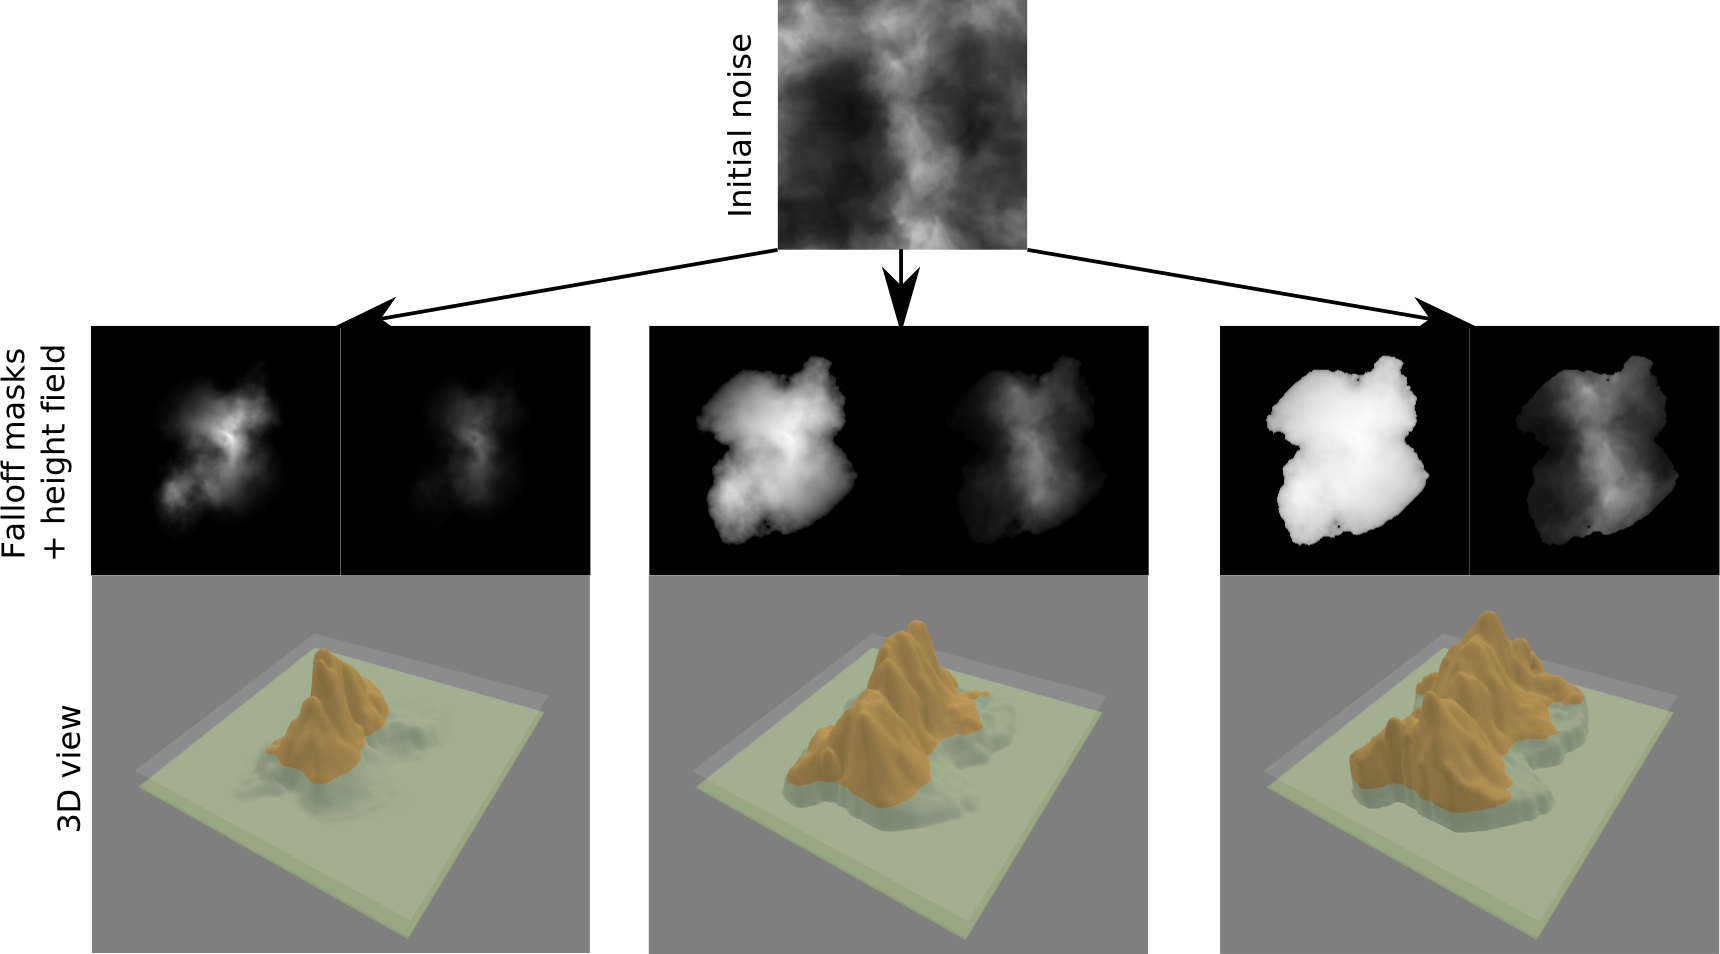
\includegraphics[width=\linewidth]{noise_examples3.pdf}
  \caption{Islands from noise + falloff (chapter example). Variations are visually diverse but lack reef semantics and controllable coastal features.}
  \label{fig:noise}
\end{figure}

\section{Overview}

\Cref{fig:pipeline} summarises the workflow. The procedural stage converts top-view outlines, a 1D elevation profile, and user strokes into a deformed height field and label map. We emulate subsidence and analytic coral growth and blend them smoothly. From randomized inputs we synthesize thousands of paired examples and augment them (translation with wrapping, rotations, flips, scaling, copy--paste). A pix2pix cGAN is trained to map HSV label maps (Hue$=$class, Value$=$subsidence) to height fields. At inference, users paint the label map; the generator produces the height field in $\sim$5\,ms on a laptop GPU.

\section{Procedural Island Generation}

\subsection{Initial Height Field from Dual-View Sketches}

The user delineates region boundaries $\{\mathcal{R}_i(\theta)\}$ in polar coordinates and specifies an elevation profile $h_{\mathrm{prof}}$ as a 1D function of a normalised ``region distance''. For pixel $p$, with polar coordinates $(r_p,\theta_p)$ about center $C$,
\begin{align}
r_p &= \|p-C\|,\qquad \theta_p = \mathrm{atan2}(p_y-C_y,\,p_x-C_x),\\
\tilde{x}_p &= i + \frac{r_p - \mathcal{R}_i(\theta_p)}{\mathcal{R}_{i+1}(\theta_p) - \mathcal{R}_i(\theta_p)} ,
\end{align}
for the unique $i$ such that $\mathcal{R}_i(\theta_p)\le r_p < \mathcal{R}_{i+1}(\theta_p)$. The base height is $h(p)=h_{\mathrm{prof}}(\tilde{x}_p)$ and the label $I(p)=i$.

\begin{figure}[t]
  \centering
  \includegraphics[width=\linewidth]{user_interaction_generation.png}
  \caption{User interface: top-view outlines (left), 1D profile (middle), and wind strokes + resistance curve (right).}
  \label{fig:ui}
\end{figure}

\subsection{Wind and Wave Deformation}

Each user stroke is a centripetal Catmull--Rom spline $\gamma$ with width $\sigma$ and strength $S_\gamma$. Let $q$ be the closest point on $\gamma$ to pixel $p$. The stroke induces a displacement
\begin{equation}
\label{eq:stroke}
w_\gamma(p) = S_\gamma\, \frac{\gamma'(q)}{\|\gamma'(q)\|}\, G_\sigma(\|p-q\|), \qquad
G_\sigma(x)=\frac{1}{\sigma\sqrt{2\pi}}e^{-x^2/(2\sigma^2)}.
\end{equation}
Aggregating all strokes and modulating by a resistance function $r(\tilde{x}_p)$ gives
\begin{equation}
\label{eq:resist}
\tilde{w}(p) = \bigl(1-r(\tilde{x}_p)\bigr)\sum_{\gamma} w_\gamma(p).
\end{equation}
We apply backward warping to height and labels:
\begin{equation}
\tilde{h}(p) = h\!\left(p-\tilde{w}(p)\right), \qquad \tilde{I}(p)=I\!\left(p-\tilde{w}(p)\right).
\end{equation}

\begin{figure}[t]
  \centering
  \includegraphics[width=.9\linewidth]{windByStrokes.pdf}
  \caption{Velocity field derived from a user stroke (red): displacement aligned with $\gamma'(q)$, decaying with Gaussian $G_\sigma$.}
  \label{fig:stroke}
\end{figure}

\subsection{Subsidence and Coral Growth}

Uniform subsidence scales the deformed surface:
\begin{equation}
h_s(p)=(1-\rho)\,\tilde{h}(p), \quad \rho\in[0,1].
\end{equation}
Coral heights are defined analytically over the reef region using smoothstep transitions. Let
\begin{equation}
\mathrm{smooth}(x)=3x^2-2x^3,\quad
S(a,b,x_0,x_1,x) = a+(b-a)\,\mathrm{smooth}\!\left(\frac{x-x_0}{x_1-x_0}\right).
\end{equation}
The piecewise function $h_c(x)$ (reef back/crest/fore with transitions) follows the chapter's definition and keeps corals near sea level.

\subsection{Smooth Maximum Blending}

We smoothly blend $h_s$ and $h_c$ using the average of under/over-estimating sigmoids (sharpness $k$):
\begin{align}
\mathrm{smx}^{-}(a,b) &= a + \frac{b-a}{1+e^{-k(b-a)}}, \quad
\mathrm{smx}^{+}(a,b) = a + \frac{b-a}{1-e^{-k(b-a)}},\\
\mathrm{smoothmax}(a,b) &= a + \frac{\mathrm{smx}^{-}(a,b)+\mathrm{smx}^{+}(a,b)}{2},
\end{align}
with continuous definition at $a=b$ as given in the chapter. The final terrain is $\hat{h}(p)=\mathrm{smoothmax}\!\bigl(h_s(p),\,h_c(p)\bigr)$.

\begin{figure}[t]
  \centering
  \includegraphics[width=.48\linewidth]{smoothmax_min-max_k-5_large.png}\hfill
  \includegraphics[width=.48\linewidth]{smoothmax_min-max_k-50_large.png}\\[0.25em]
  \includegraphics[width=.48\linewidth]{smoothmax_min-max_k-5_short.png}\hfill
  \includegraphics[width=.48\linewidth]{smoothmax_min-max_k-50_short.png}
  \caption{Smooth maximum behaviour for different $k$ (chapter figures).}
  \label{fig:smoothmax}
\end{figure}

\section{Dataset Synthesis and Augmentation}

We randomize outlines, profile, and resistance with bounded Perlin/fBm noise; generate 2--6 random wind strokes and thin radial strokes for drainage-like features; and export multiple subsidence levels per island.
%
Inputs are stored as HSV images with Hue$=$class label and Value$=\rho$ (Saturation neutral). Targets are RGB height fields. Augmentation includes translation with wrapping, rotations, flips, scalings, and copy--paste of multiple islands with smoothmax height blending and $\max$ label blending.

\section{Learning with pix2pix}

We train pix2pix~\cite{Isola2017}: U-Net generator with PatchGAN discriminator, adversarial + $\ell_1$ loss ($\lambda{=}100$), Adam optimizer (lr=0.0002, $\beta_1{=}0.5$, $\beta_2{=}0.999$), batch size 1. From $\sim$1\,000 base islands, augmentation yields $\sim$10\,000 samples per epoch; grid artifacts largely disappear after the second epoch. At test time, painting a $256{\times}256$ HSV label map yields height maps in $\sim$5\,ms on a GTX~1650~Ti; optimized C++ procedural generation runs in $\sim$50\,ms per island.

\begin{figure}[t]
  \centering
  \includegraphics[width=.95\linewidth]{user_interaction_generation.png}\\[-0.25em]
  \includegraphics[width=.95\linewidth]{other_images/Drawings/Darwin_corals-color-Terry2012.jpg}
  \caption{Top: editing canvases (labels, profile, strokes, resistance). Bottom: classical Darwin subsidence illustration used for context in the chapter.}
  \label{fig:context}
\end{figure}

\section{Results}

Qualitative outputs show plausible coral morphologies from rough or fuzzy sketches, with robust handling of inconsistent pixels (e.g., abyss near beach). Style can be steered by retraining on a ``volcanic'' procedural dataset (lower reef resistance, central crater). The learned model breaks radial symmetry present in procedural-only outputs and maintains semantic consistency, enabling texturing and instance placement by region.

\begin{figure}[t]
  \centering
  \includegraphics[width=.49\linewidth]{example_pix2pix_facade.png}\hfill
  \includegraphics[width=.49\linewidth]{example_pix2pix_maps.png}
  \caption{Image-to-image conditioning paradigm (pix2pix examples from chapter): we apply the same idea to map label maps to height fields.}
  \label{fig:pix2pix}
\end{figure}

\paragraph{Performance.} Inference: $\sim$5\,ms per $256^2$ image on GTX~1650~Ti; dataset synthesis (optimized): $\sim$50\,ms per island. Training converges to artifact-free results in under ten epochs on our synthetic dataset.

\section{Discussion}

\textbf{Advantages.} The hybrid approach provides (i) controllable large-scale structure via sketches, (ii) learned detail and asymmetry beyond procedural biases, (iii) no reliance on scarce real DEMs, (iv) preserved labels for downstream operations, and (v) real-time feedback.

\textbf{Limitations.} The cGAN inherits biases from the procedural dataset; out-of-distribution layouts degrade quality; resolution is limited to $256^2$; user control during inference is indirect (via label maps and global subsidence).

\section{Conclusion and Future Work}

We introduced a procedural-to-learning pipeline for coral reef islands that leverages domain-inspired rules to synthesize training data for a cGAN. The system generates plausible terrains from simple semantic sketches at interactive rates. Future directions include conditioning on wind vector fields, increasing user control at inference, and extending the procedural model with higher-fidelity erosion/tidal dynamics; style-transfer or super-resolution models could increase detail without sacrificing speed.

\paragraph{Reproducibility.} We follow the chapter's implementation; releasing scripts for dataset generation, training configuration, and pretrained weights is straightforward.

% \bibliographystyle{unsrt}
% % Use the same .bib file as your thesis; keys are unchanged.
% \bibliography{YOUR_BIB_FILE_NAME}

% \end{document}
